\chapter{Web Application}

\section{Task Assignment and Completion}

\begin{table}[h]
\centering
\begin{tabular}{|l|p{9cm}|c|}
\hline
\textbf{Member} & \textbf{Responsibilities} & \textbf{Completed Rate} \\ \hline

Dang Truong Nguyen
& Frontend (HTML, CSS, JS) and Backend (Lambda CRUD APIs, DynamoDB integration); IAM Roles configuration and API testing 
& 100\% \\ \hline

Nguyen Thanh Gia Bao 
& Networking setup: VPC, Private Subnets, VPC Endpoint for DynamoDB, Lambda VpcConfig, Route Table; collect NE evidence 
& 100\% \\ \hline

Le Tuan Loc
& Deployment and Security: S3 private, CloudFront + OAC, API Gateway (CORS, throttling); Monitoring (CloudWatch, Alarms, Budget); collect SE and IM evidence 
& 100\% \\ \hline

\end{tabular}
\caption{Team Contribution}
\end{table}

\section{Frontend accessible via the CloudFront URL}
\begin{itemize}
    \item \textbf{Serverless Application URL:} \url{https://d14g6okcs1rawz.cloudfront.net/index.html}
\end{itemize}

\section{Backend API}
\begin{itemize}
    \item \textbf{Backend API accessible via the API gateway URL:} \url{https://py29vzblk3.execute-api.ap-southeast-2.amazonaws.com/prod}
\end{itemize}

\subsection{API \texttt{GET /tasks} testing with Postman}
\begin{figure}[H]
    \centering
    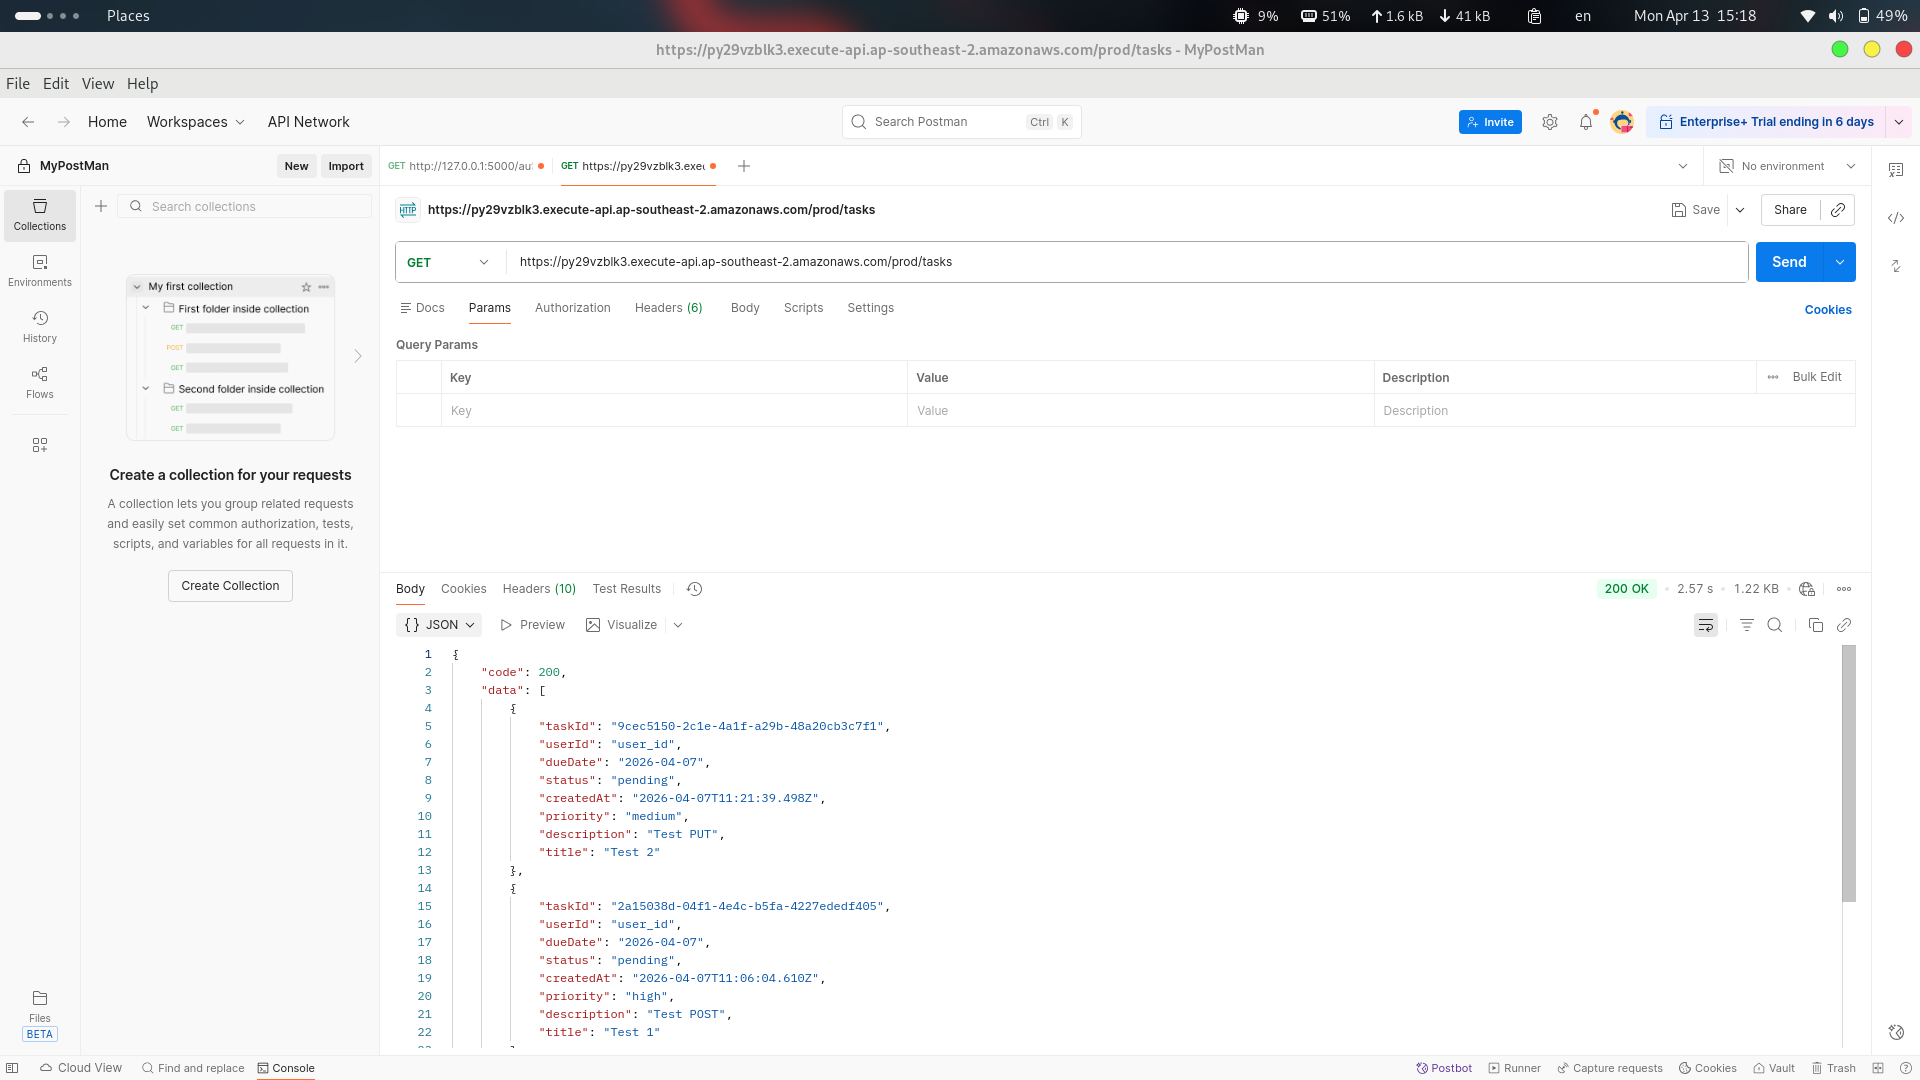
\includegraphics[width=0.8\textwidth]{images/API1.png}
    \caption{\texttt{GET /tasks}}
\end{figure}

\subsection{API \texttt{POST /tasks} testing with Postman}
\begin{figure}[H]
    \centering
    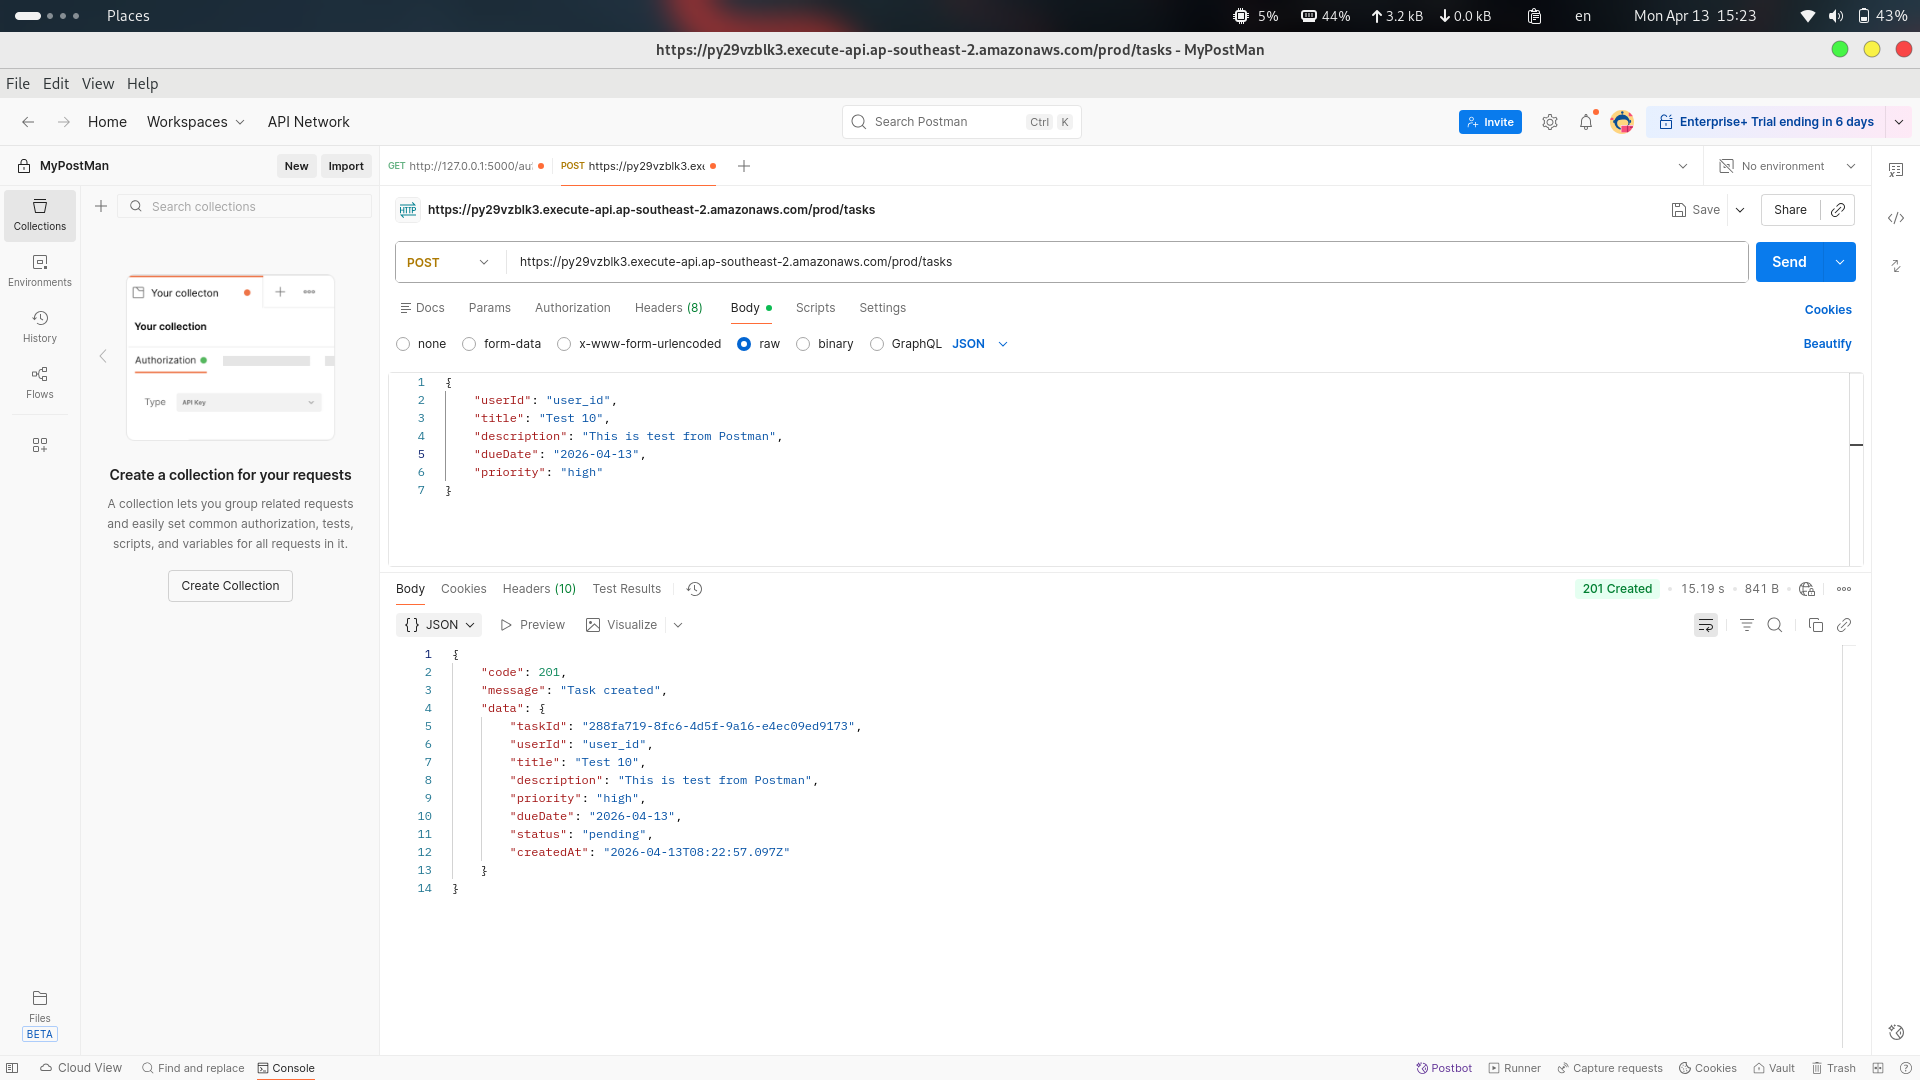
\includegraphics[width=0.8\textwidth]{images/API2.png}
    \caption{\texttt{POST /tasks}}
\end{figure}

\subsection{API \texttt{PUT /tasks/{id}} testing with Postman}
\begin{figure}[H]
    \centering
    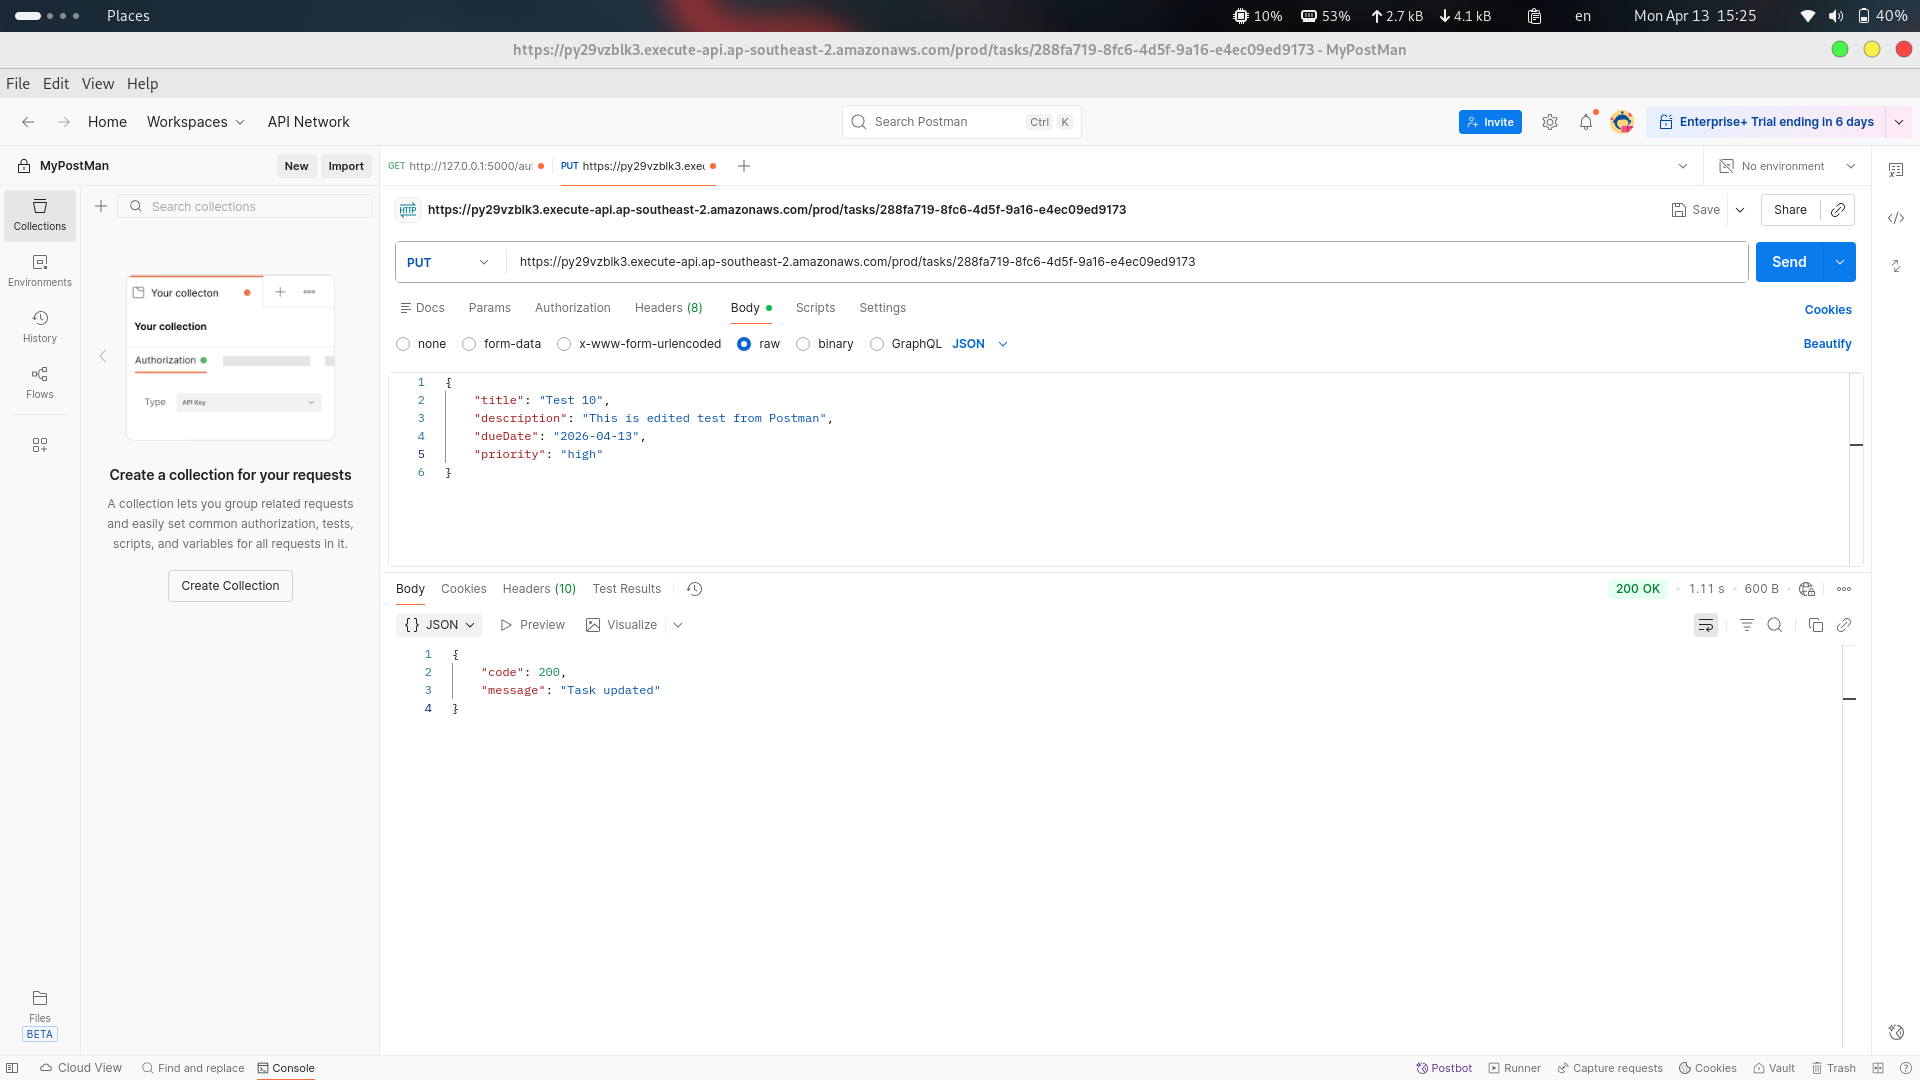
\includegraphics[width=0.8\textwidth]{images/API3.png}
    \caption{\texttt{PUT /tasks/{id}}}
\end{figure}

\subsection{API \texttt{DELETE /tasks/{id}} testing with Postman}
\begin{figure}[H]
    \centering
    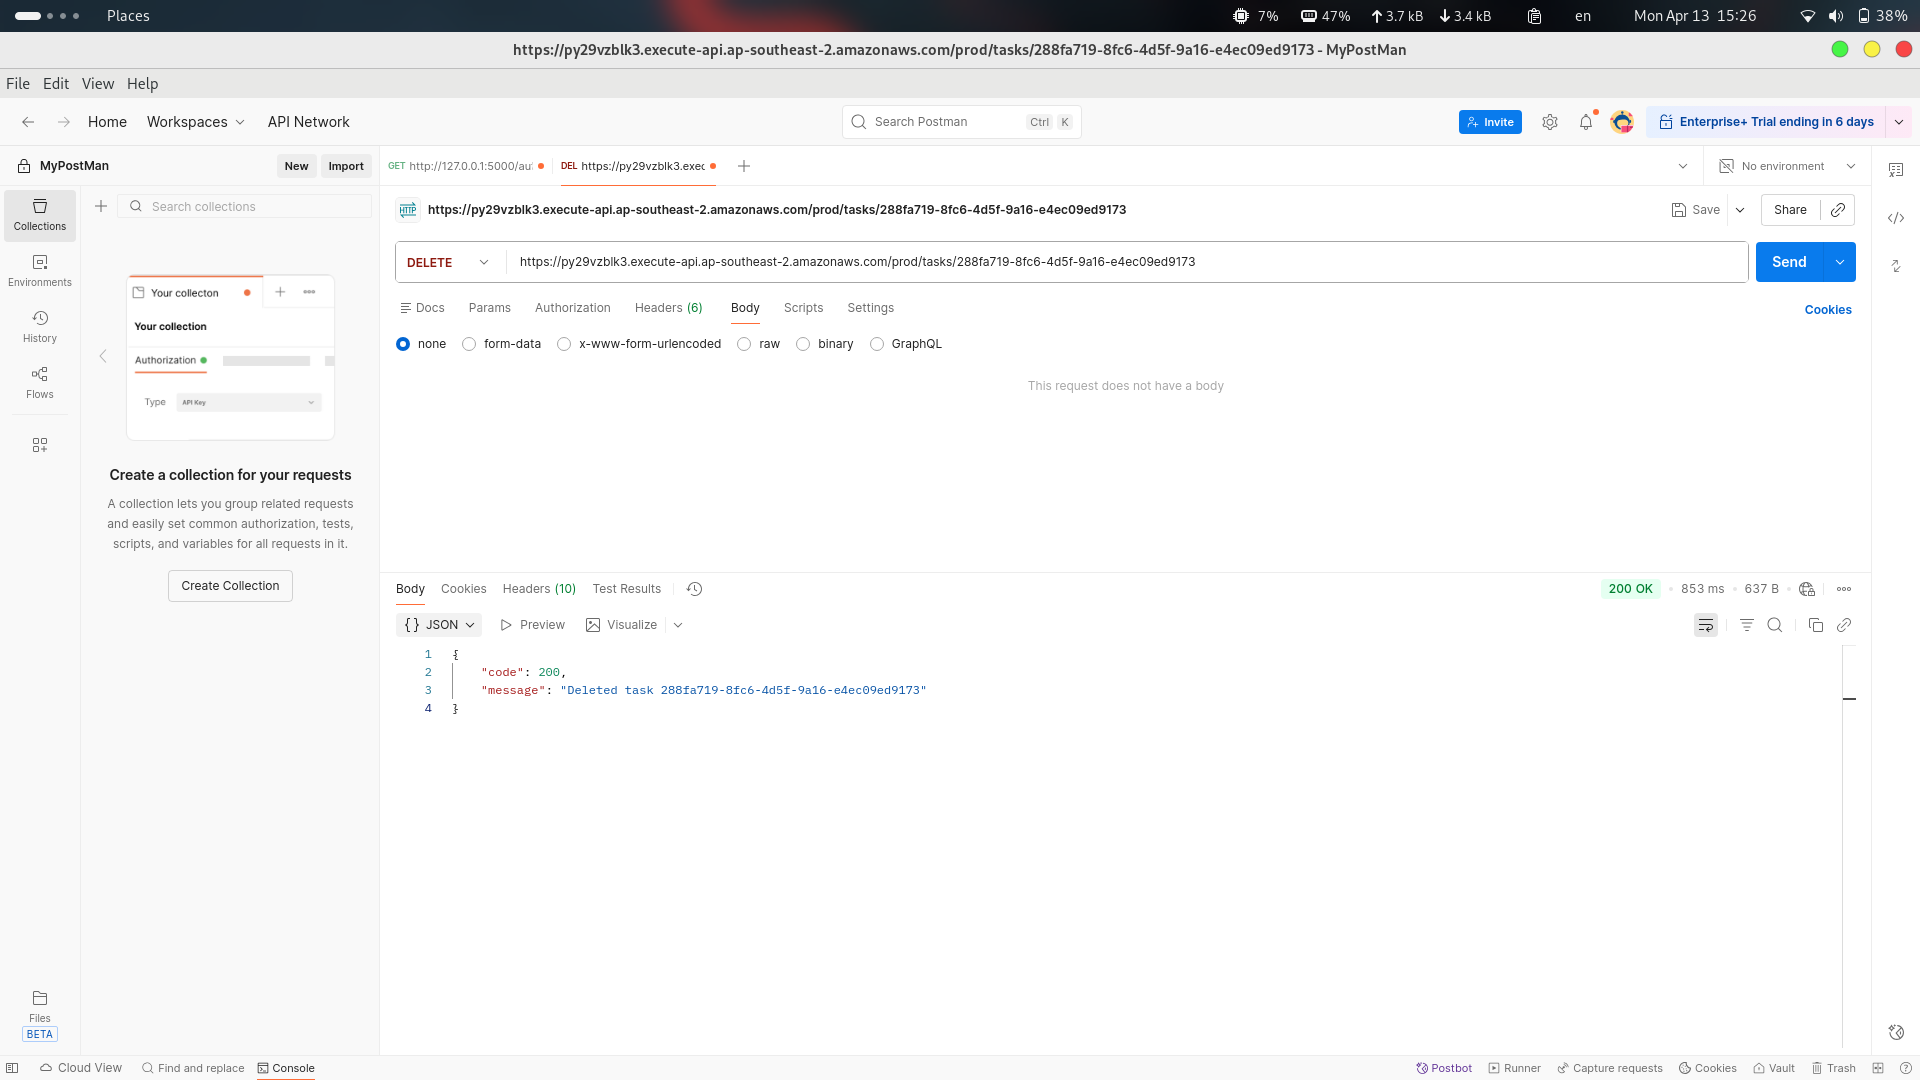
\includegraphics[width=0.8\textwidth]{images/API4.png}
    \caption{\texttt{DELETE /tasks/{id}}}
\end{figure}

\section{Database Item}
\begin{figure}[H]
    \centering
    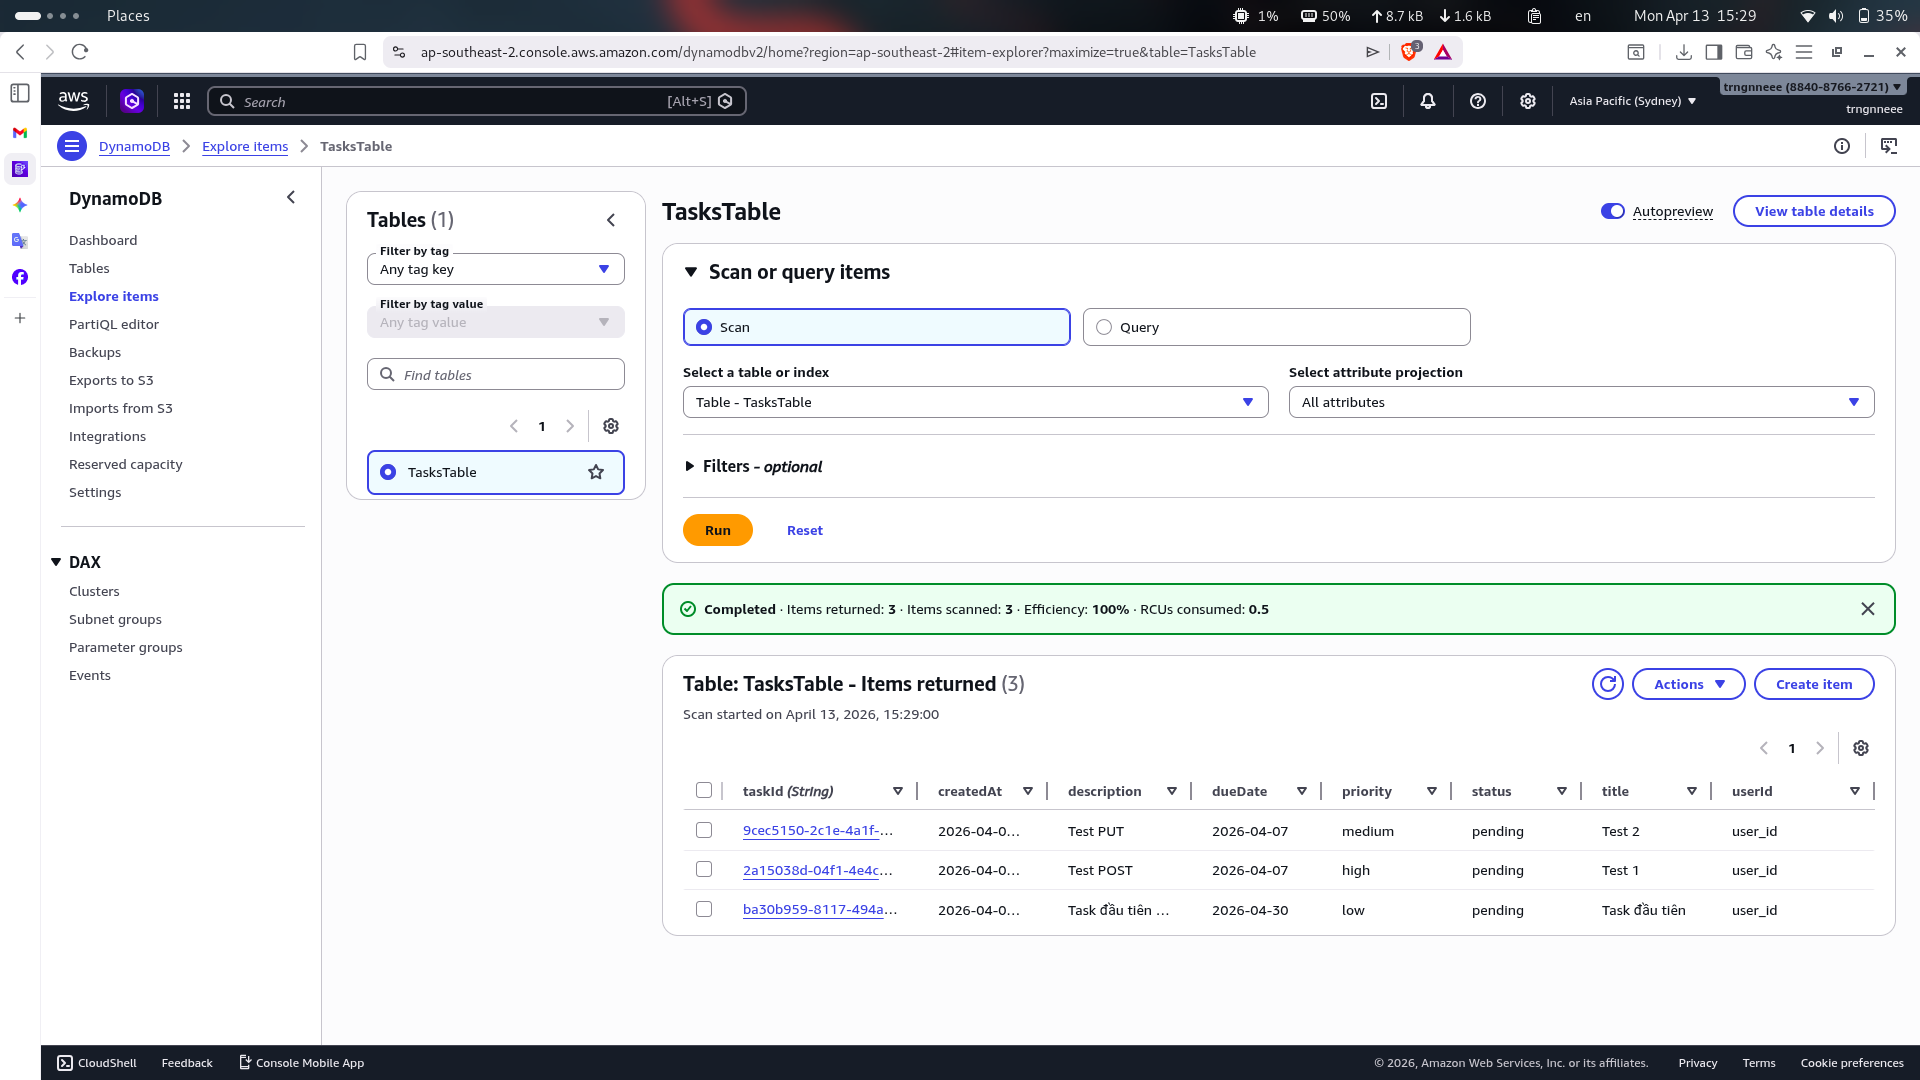
\includegraphics[width=0.8\textwidth]{images/DB.png}
    \caption{Database Explorer}
\end{figure}
